\documentclass[submit]{../harvardml}

\course{CS1810-S25}
\assignment{Homework \#4}
\duedate{April 4, 2025 at 11:59 PM}

\usepackage[OT1]{fontenc}
\usepackage[colorlinks,citecolor=blue,urlcolor=blue]{hyperref}
\usepackage[pdftex]{graphicx}
\usepackage{graphicx}
\usepackage{caption}
\usepackage{fullpage}
\usepackage{soul}
\usepackage{amsmath}
\usepackage{amssymb}
\usepackage{framed}
\usepackage{color}
\usepackage{todonotes}
\usepackage{listings}
\usepackage{../common}
\usepackage{xcolor}
\usepackage{float}
%%%%%%%%%%%%%%%%%%%%%%%%%%%%%%%%%%%%%%%%%%%
%% Solution environment
\usepackage{xcolor}
\newenvironment{solution}{
    \vspace{2mm}
    \color{blue}\noindent\textbf{Solution}:
}{}
%%%%%%%%%%%%%%%%%%%%%%%%%%%%%%%%%%%%%%%%%%%

\usepackage[mmddyyyy,hhmmss]{datetime}

\definecolor{verbgray}{gray}{0.9}

\lstnewenvironment{csv}{
  \lstset{backgroundcolor=\color{verbgray},
  frame=single,
  framerule=0pt,
  basicstyle=\ttfamily,
  columns=fullflexible}}{}
 
\begin{document}

\begin{center}
{\Large SVM, Clustering, and In-Depth Ethics}\\
\end{center}

\subsection*{Introduction}

This homework assignment will have you work with SVMs, clustering, and engage with the ethics lecture.

\subsection*{Resources and Submission Instructions}
We encourage you to
read Chapter 5 in the textbook to learn more about SVMs, 6.2 to review k-means clustering, and 6.3 to review HAC. % FDV (done): Fill from textbook \

Please submit the \textbf{writeup PDF to the Gradescope assignment `HW4'}. Remember to assign pages for each question.

Please submit your \textbf{\LaTeX\ file and code files to the Gradescope assignment `HW4 - Supplemental'}. 

You can use a \textbf{maximum of 2 late days} on this assignment.  Late days will be counted based on the latest of your submissions. 

\newpage

%%%%%%%%%%%%%%%%%%%%%%%%%%%%%%%%%%%%%%%%%%%%%
% Problem 1
%%%%%%%%%%%%%%%%%%%%%%%%%%%%%%%%%%%%%%%%%%%%%
\begin{problem}[Fitting an SVM by hand, 10pts]
  For this problem you will solve an SVM by hand, relying on principled rules and SVM properties. 
  For making plots, however, you are allowed to use a computer or other graphical tools.

  Consider a dataset with the following 7 data points each with $x \in \reals$ and $y \in \{ -1, +1 \}$ : \[\{(x_i, y_i)\}_{i = 1}^7 =\{(-3 , +1) , (-2 , +1 ) , (-1,  -1 ), (0, +1), ( 1 , -1 ), ( 2 , +1 ) , (3 , +1 )\}\] Consider
  mapping these points to $2$ dimensions using the feature vector $\bphi(x) =  (x, -\frac{8}{3}x^2 + \frac{2}{3}x^4)$. The hard margin classifier training problem is:
  \begin{align*}
    &\min_{\mathbf{w}, w_0} \frac{1}{2}\|\mathbf{w}\|_2^2 \label{eq:dcp} \\
    \quad \text{s.t.} \quad & y_i(\mathbf{w}^\top \bphi(x_i) + w_0) \geq 1,~\forall i \in \{1,\ldots, n\}\notag
  \end{align*}

  Make sure to follow the logical structure of
  the questions below when composing your answers, and to justify each step.

  \begin{enumerate}
    \item Plot the transformed training data in $\reals^2$ and draw the optimal decision boundary
    of the max margin classifier. You can determine this by inspection (i.e. by hand, without actually doing any calculations).

    \item What is the value of the margin achieved by the optimal
    decision boundary found in Part 1? 

    \item Identify a unit vector that is orthogonal to the decision boundary.

    \item Considering the discriminant $h(\bphi(x);\boldw,w_0)=\boldw^\top\bphi(x) +w_0$, 
    give an expression for {\em all possible} $(\boldw,w_0)$ that define
    the decision boundary. Justify your answer.

    \item Consider now the training problem for this dataset. Using your answers so far,
    what particular solution to $\boldw$ will be optimal for the
    optimization problem?

    \item What is the corresponding optimal value of $w_0$ for the $\boldw$ found in Part 5 (use your result from Part 4 as guidance)? Substitute in these optimal values and write out the discriminant function
    $h(\bphi(x);\boldw,w_0)$ in terms of the variable $x$.

    \item Which points could possibly be support vectors of the classifier?  Confirm that
    your solution in Part 6 makes the constraints above tight---that is,
    met with equality---for these candidate points.

    \item Suppose that we had decided to use a different feature mapping
    $\bphi'(x) = (x, -\frac{31}{12}x^2 + \frac{7}{12}x^4 )$.  Does
    this feature mapping still admit a separable solution?  How does
    its margin compare to the margin in the previous parts?  Based on
    this, which set of features might you prefer and why?   
  \end{enumerate}
\end{problem}
\newpage
\begin{solution}
\\
\textbf{1.} By inspection, the optimal decision boundary of the SVM should be the horizontal line $\phi_2(x) = -1$ which evenly splits the blue and red points near the bottom of the graph.
\begin{figure}[H]
    \centering
    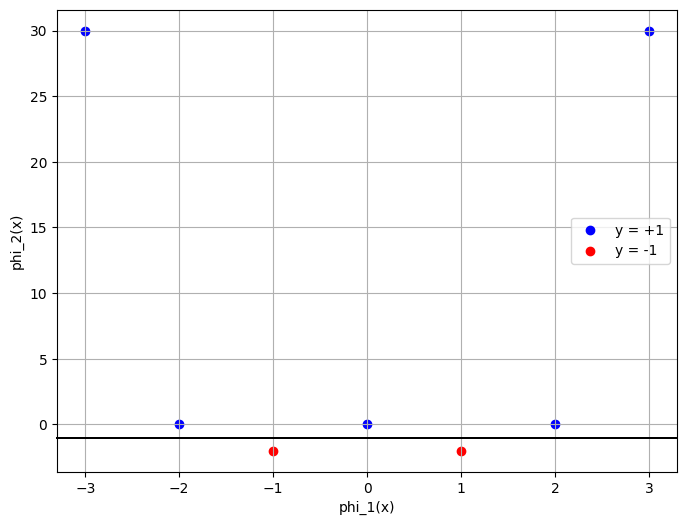
\includegraphics[width=0.8\linewidth]{hw4/img_output/p1.1.png}
\end{figure}
\textbf{2.} The value of the margin achieved by the optimal decision boundary from part (1) is $1$. This is because the blue support vectors are at $\phi_2(x) = 0$ and the red support vectors are at $\phi_2(x) = -2$, so the orthogonal distance of the horizontal boundary splitting these points is $1$. 
\\
\\
\textbf{3.} Since the decision boundary is a horizontal line, any vertical vector (pointing in the direction of $\phi_2(x)$) is orthogonal. Therefore, a unit vetor that is orthogonal to the decision boundary is $v_{\phi(x)} = [0,1]$.
\\
\\
\textbf{4.} On the decision boundary, we have by definition that
$$h(\bphi(x);\boldw,w_0)=\boldw^\top\bphi(x) +w_0 = 0$$
Moreover, from the textbook, we know that $\boldw$ must be orthogonal to this hyperplane. Thus, from part (3), we know that $\boldw$ must take the form of
$$\boldw = (0,a) \quad a \in \mathbb{R}$$
Then, since we determined in part (1) that the optimal decision boundary is the horizontal line $\phi_2(x) = -1$, 
$$\boldw^\top\bphi(x) +w_0 = a \phi_2(x) + w_0 = -a + w_0 = 0 \quad \longrightarrow \quad w_0 = a$$
Therefore, all $(\boldw, w_0)$ are of the form $((0,a),a)$ with $a \in \mathbb{R}$
\\
\\
\textbf{5.} Since $\boldw$ must be of the form $(0,a)$, the SVM objective is to minimize 
$$\frac{1}{2}\|\boldw\|_2^2 = \frac{1}{2}a^2$$  
Subject to the constraints 
$$y_i\Bigl(\boldw^\top\bphi(x_i) +w_0\Bigr) \ge 1$$
Thus, for the positive support vectors at $\phi_2(x)=0$, the constraint is  
$$+1\Bigl(a\cdot 0+w_0\Bigr)=w_0\ge 1$$  
For the negative support vectors at $\phi_2(x)=-2$, the constraint becomes  
$$-1\Bigl(a\cdot (-2)+w_0\Bigr)=2a-w_0\ge 1$$  
Recall from part (4) we have $w_0=a$. Thus, substituting gives $a\ge 1$ from both constraints (for the positive case $a\ge1$ and for the negative case $2a-a = a\ge1$). To minimize $\frac{1}{2}a^2$, we choose the smallest $a$ satisfying these constraints, namely $a=1$. Therefore, the optimal $\boldw$ of form $(0,a)$ is
$$\boldw=(0,1)$$
\\
\textbf{6.} Recall from part (4) that $w_0 = a$ and we found in part (5) that $a=1$ is optimal. Therefore, the optimal value of $w_0$ for the $\boldw$ found in part (5) is
$$w_0 = 1$$
Substituting these values into the discriminant function gives  
$$h(\bphi(x);\boldw,w_0)=\phi_2(x)+1$$  
Then, since  
$$\phi_2(x)=-\frac{8}{3}x^2+\frac{2}{3}x^4$$  
We have  the discriminant function as
$$h(x)=-\frac{8}{3}x^2+\frac{2}{3}x^4+1$$
\textbf{7.} Based on the plot, the points $(-2,1)$, $(-1,-1)$, $(0,1)$, $(1,-1)$, and $(2,1)$ lie closest to the decision boundary and are candidate support vectors, while $(-3,1)$ and $(3,1)$ are clearly farther away and thus are not candidates. The support vectors must satisfy (making the constraints tight)
$$y_i\Bigl(\boldw ^\top\phi(x_i)+1\Bigr)= y_i\Bigl(\phi_2(x_i)+1\Bigr)=1$$  
For $x = -2$ with $y = 1$, we have 
$$\phi_2(-2) = -\frac{8}{3}(4) + \frac{2}{3}(16) = 0 \quad \longrightarrow \quad +1(0+1)=1$$ 
For $x = 0$ with $y = 1$, 
$$\phi_2(0)= 0 \quad \longrightarrow \quad +1(0+1)=1$$ 
For $x = 2$ with $y = 1$, 
$$\phi_2(2)= -\frac{8}{3}(4) + \frac{2}{3}(16) = 0 \quad \longrightarrow \quad +1(0+1)=1$$ 
For $x = -1$ with $y = -1$, 
$$\phi_2(-1) = -\frac{8}{3}(1) + \frac{2}{3}(1) = -2 \quad \longrightarrow \quad -1(-2+1)=1$$ 
For $x = 1$ with $y = -1$, 
$$\phi_2(1) = -2 \quad \longrightarrow \quad -1(-2+1)=1$$ 
Thus, the margin constraint is tight for all of our candidate points.
\\
\\
\textbf{8.}  Using the alternative feature mapping 
$$
\bphi'(x)=\Bigl(x,\; -\frac{31}{12}x^2+\frac{7}{12}x^4\Bigr),
$$ 
the data remain separable as shown in the line I drew. However, visually the classes are closer together, resulting in a smaller margin of approximately $0.5$ compared to the margin of $1$ obtained with the original mapping. Since a larger margin usually leads to better generalization, I would choose the original set of features over the alternative feature mapping.
\begin{figure}[H]
    \centering
    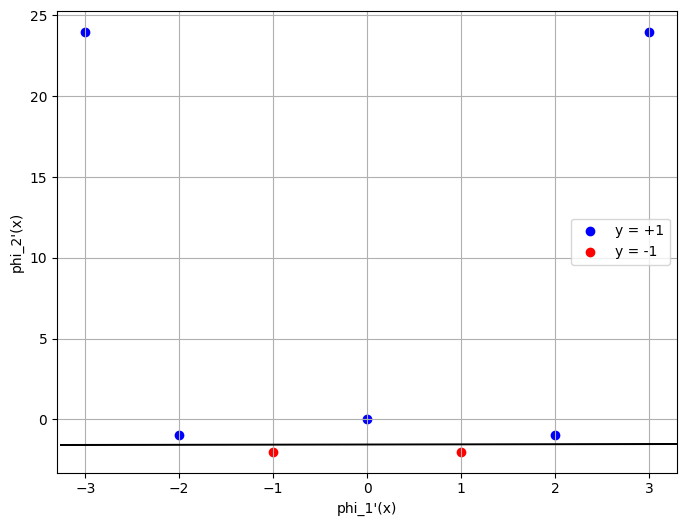
\includegraphics[width=0.8\linewidth]{hw4/img_output/p1.8.png}
    \caption{Caption}
    \label{fig:enter-label}
\end{figure}
\end{solution}


\newpage

%%%%%%%%%%%%%%%%%%%%%%%%%%%%%%%%%%%%%%%%%%%%%
% Problem 2
%%%%%%%%%%%%%%%%%%%%%%%%%%%%%%%%%%%%%%%%%%%

\begin{problem}[K-Means and HAC, 20pts]

  For this problem you will implement K-Means and HAC from scratch to cluster image data. You may use \texttt{numpy} but no third-party ML implementations (eg. \texttt{scikit-learn}).

  Your job is to implement K-means and HAC on MNIST, a collection of handwritten digits, and to test whether these relatively simple algorithms can cluster similar-looking images together.

  The code in \texttt{homework4.ipynb} loads the images into your environment into two arrays -- \texttt{large\_dataset}, a 5000x784 array, will be used for K-means, while \texttt{small\_dataset}, a 300x784 array, will be used for HAC. In your code, you should use the $\ell_2$ norm (i.e. Euclidean distance) as your distance metric.

  \textbf{Important:} Remember to include all of your plots in your PDF submission!

  \begin{enumerate}
    \item Starting at a random initialization and $K = 10$, plot the
      K-means objective function (the residual sum of squares) as a
      function of iterations and verify that it never increases.

    \item For $K=10$ and for 3 random restarts, print the mean image (aka
      the centroid) for each cluster. There should be 30 total images.

    \item Repeat Part 2, but before running K-means, standardize or center
      the data such that each pixel has mean 0 and variance 1 (for any
      pixels with zero variance, simply divide by 1). For $K=10$ and 3
      random restarts, show the mean image (centroid) for each
      cluster. Again, present the 30 total images in a single
      plot. Compare to Part 2: How do the centroids visually differ? Why?

    \item Implement HAC for min, max, and centroid-based linkages. Fit
      these models to the \texttt{small\_dataset}.  For each of these 3
      linkage criteria, find the mean image for each cluster when using
      $10$ clusters. Display these images (30 total) on a single plot.

      How do the ``crispness'' of the cluster means and the digits
      represented compare to mean images for k-means?  
      Why do we only ask you to run HAC once?  

      \textbf{Important Note:} For this part ONLY, you may use
      \texttt{scipy}'s \texttt{cdist} function to calculate Euclidean
      distances between every pair of points in two arrays.

    \item For each of the HAC linkages, as well as one of the runs of your
      k-means, make a plot of ``Number of images in cluster" (y-axis)
      v. ``Cluster index" (x-axis) reflecting the assignments during the
      phase of the algorithm when there were $K=10$ clusters.

      Intuitively, what do these plots tell you about the difference
      between the clusters produced by the max and min linkage criteria?

      Going back to the previous part: How does this help explain the
      crispness and blurriness of some of the clusters?  
  \end{enumerate}
\end{problem}
\newpage
\begin{framed}
  \noindent\textbf{Problem 2} (cont.)\\
  \begin{enumerate}
  \setcounter{enumi}{5}
    \item For your K-means with $K = 10$ model and HAC min/max/centroid
      models using $10$ clusters on the \texttt{small\_dataset} images,
      use the \texttt{seaborn} module's \texttt{heatmap} function to plot
      a confusion matrix between each pair of clustering methods.  This
      will produce 6 matrices, one per pair of methods. The cell at the
      $i$th row, $j$th column of your confusion matrix is the number of
      times that an image with the cluster label $j$ of one method has
      cluster $i$ in the second method.  Which HAC is closest to k-means?
      Why might that be?

    \item Let's return to the postal service example from HW3.  Do you
      think that clustering is a good way to identify digits, that is,
      first cluster the data, and then, for any new data point, classify
      it based on its cluster?
      \begin{enumerate}
        \item In particular, do you expect the clusters to correspond with the
          true labels?  Is that a good way to evaluate clustering?
        
        \item In previous homeworks, you considered the possibility of adversarial attacks. 
        In a similar vein of thought, discuss some types of ``bad'' data that clustering algorithms 
        in particular may struggle to handle. For example, what might happen if you run clustering algorithms
        on a dataset with a few noisy outliers that are far from the rest of the dataset?
      \end{enumerate}
  \end{enumerate}
\end{framed}

\begin{solution}
    \\
    \textbf{1. } As we can see below, the K-means objective function never increases (monotonically decreasing).
    \begin{figure}[H]
        \centering
        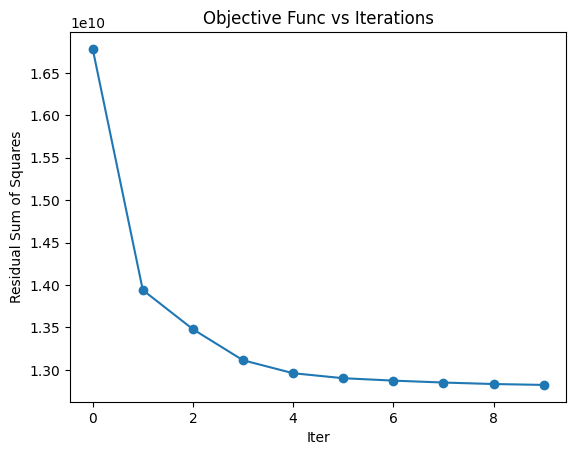
\includegraphics[width=0.8\linewidth]{hw4/img_output/p2.1.png}
    \end{figure}
    \textbf{2.} 
    \begin{figure}[H]
        \centering
        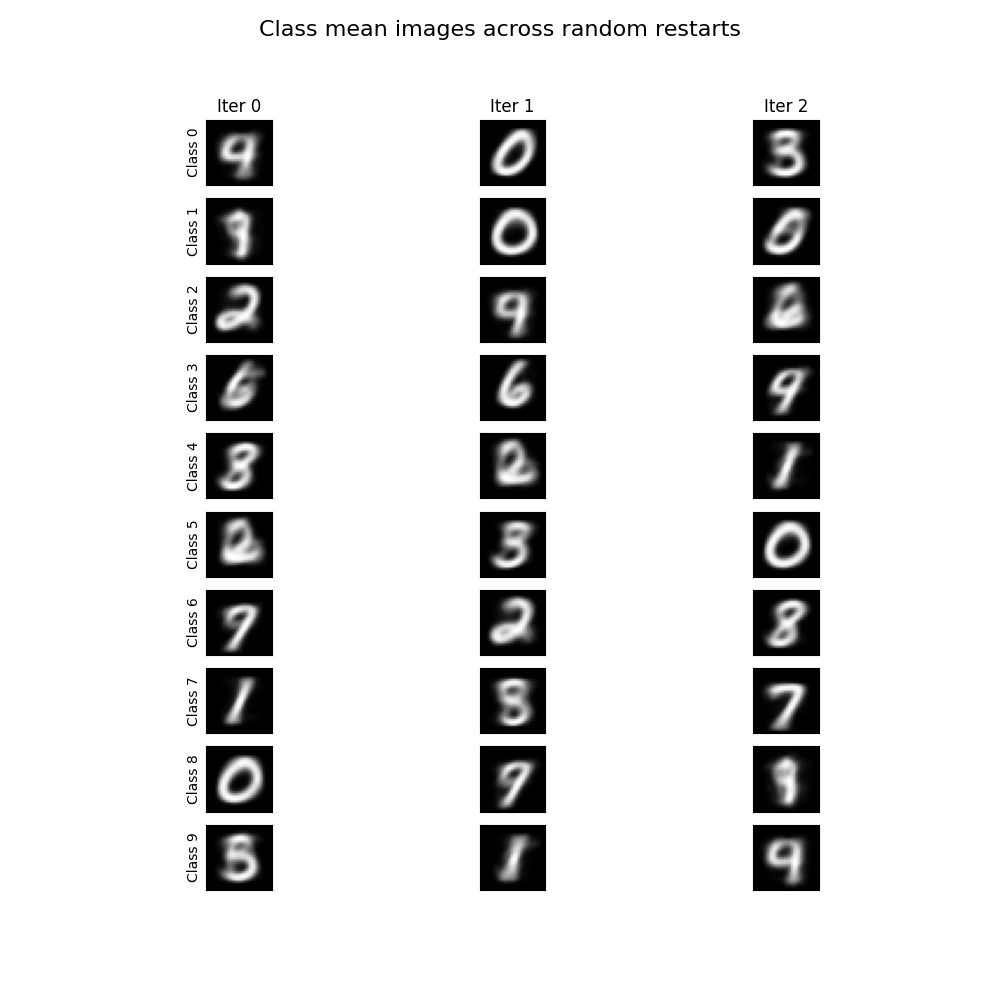
\includegraphics[width=0.6\linewidth]{hw4/img_output/p2.2.png}
    \end{figure}
    \textbf{3.} The centroids look less defined and more blurry compared to the centroids of the non-standardized data. The distinguishability of the standardized centroids is much worse the non-standardized data, and most appear more gray compared to part (2). This is because standardization removes the original brightness and contrast of each pixel, forcing all pixels to have the same mean and variance across images. As a result, when we average the images to compute centroids, the details get washed out and the digit shapes become less distinct. In contrast, the non-standardized data preserves natural pixel intensity patterns, making the centroids sharper and more recognizable.
    \begin{figure}[H]
        \centering
        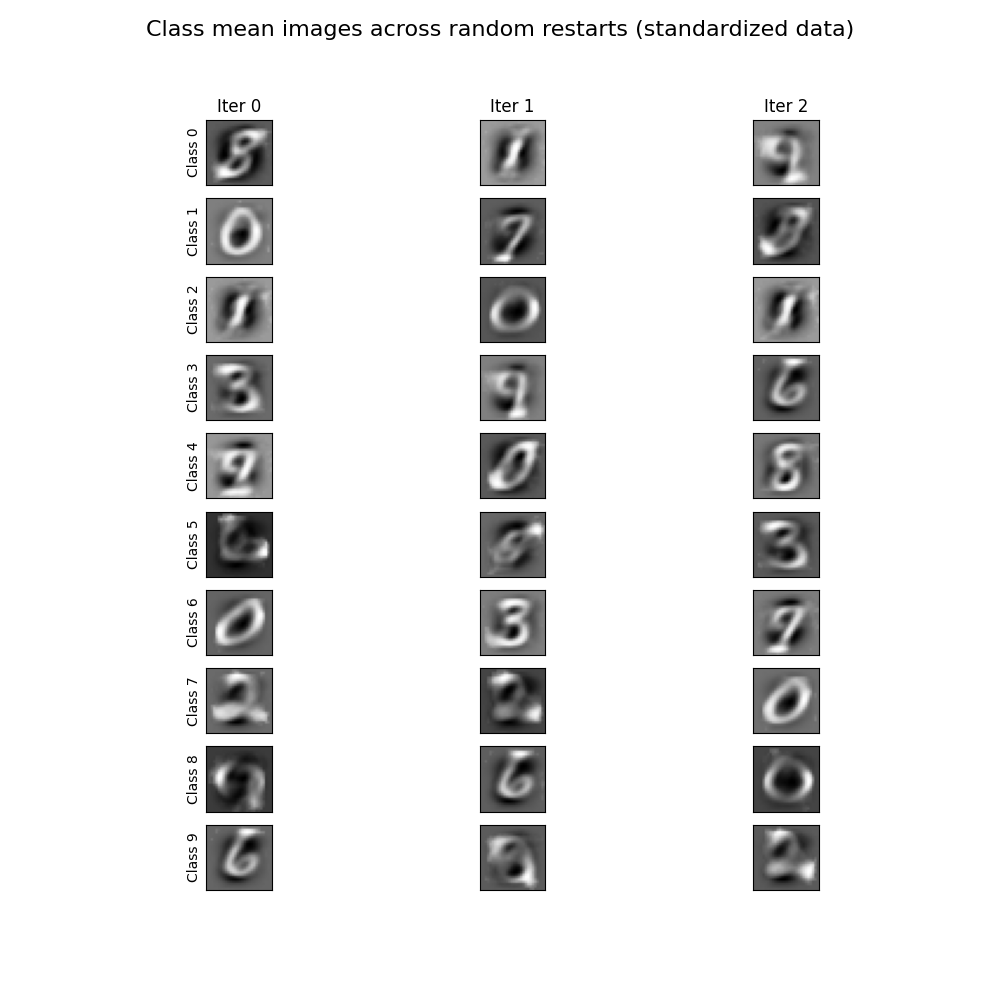
\includegraphics[width=0.6\linewidth]{hw4/img_output/p2.3.png}
    \end{figure}
    \textbf{4.} The min and centroid linkage images are generally a little more crisp compared to the K-Means images, with the min linkage images being the most crisp. However, many of the digits are not represented in the images, with digits like 2 being repeated many times. Thus, while the crispness for the min and centroid linkage is a little better than K-Means, the representation of digits is far worse. The max linkage images are the blurriest out of all the HAC images and are considerably less crisp than K-Means. However, the representation of digits appears to be much better than in the min and centroid images, comparable to the K-Means representation.
    \\
    \\
    We only need to run HAC once for each linkage criterion because the algorithm is deterministic. Unlike K-Means, there are no random initializations, so we get the same results each time.
    \begin{figure}[H]
        \centering
        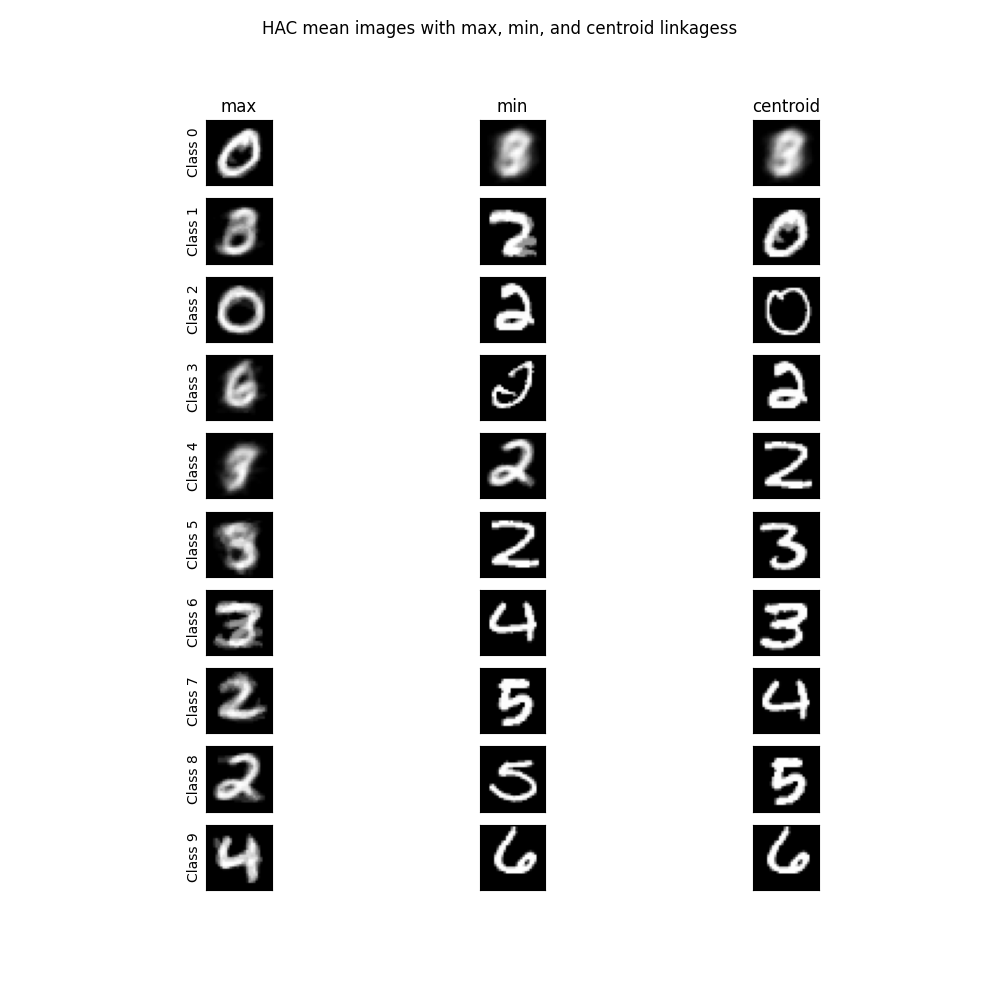
\includegraphics[width=0.6\linewidth]{hw4/img_output/p2.4.png}
    \end{figure}
    \textbf{5.} From the cluster size plots, we see that min linkage can accumulate many points into a single large cluster, leaving only a few smaller ones. This is because min linkage merges clusters whose closest pair of points is minimal, so a cluster can repeatedly attract nearby points which causes it to grow extremely fast and dominate. On the other hand, max linkage merges clusters based on their farthest pair of points, which limits the formation of a dominant cluster and thus results in a more balanced distribution of cluster sizes. As such, large clusters tend to produce blurrier mean images (since they average over many different examples), while smaller clusters yield sharper, more defined centroids, which we observed in the previous part.
    \begin{figure}[H]
        \centering
        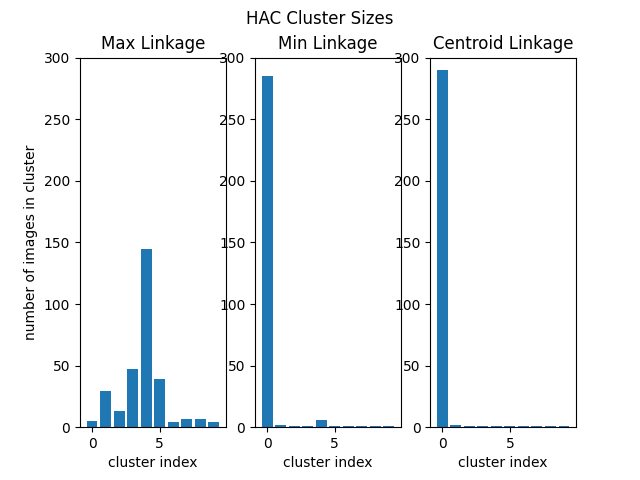
\includegraphics[width=0.8\linewidth]{hw4/img_output/p2.5a.png}
    \end{figure}
    \begin{figure}[H]
        \centering
        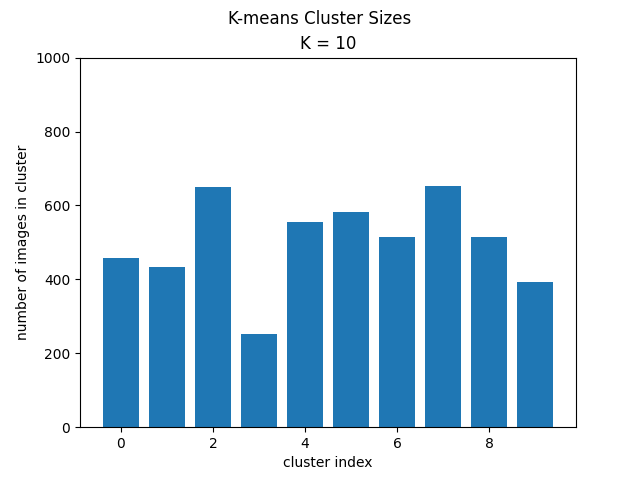
\includegraphics[width=0.8\linewidth]{hw4/img_output/p2.5b.png}
    \end{figure}
    \textbf{6.} The confusion matrices show that HAC with max linkage aligns most closely with K-Means. Both methods favor compact, spherical clusters, since K-Means averages points into centroids and max linkage merges clusters based on the maximum pairwise distance (therefore discouraging large clusters). This shared tendency for compact grouping leads to similar cluster assignments, as we can see by the high overlap in their confusion matrices.
 
    \begin{figure}[H]
        \centering
        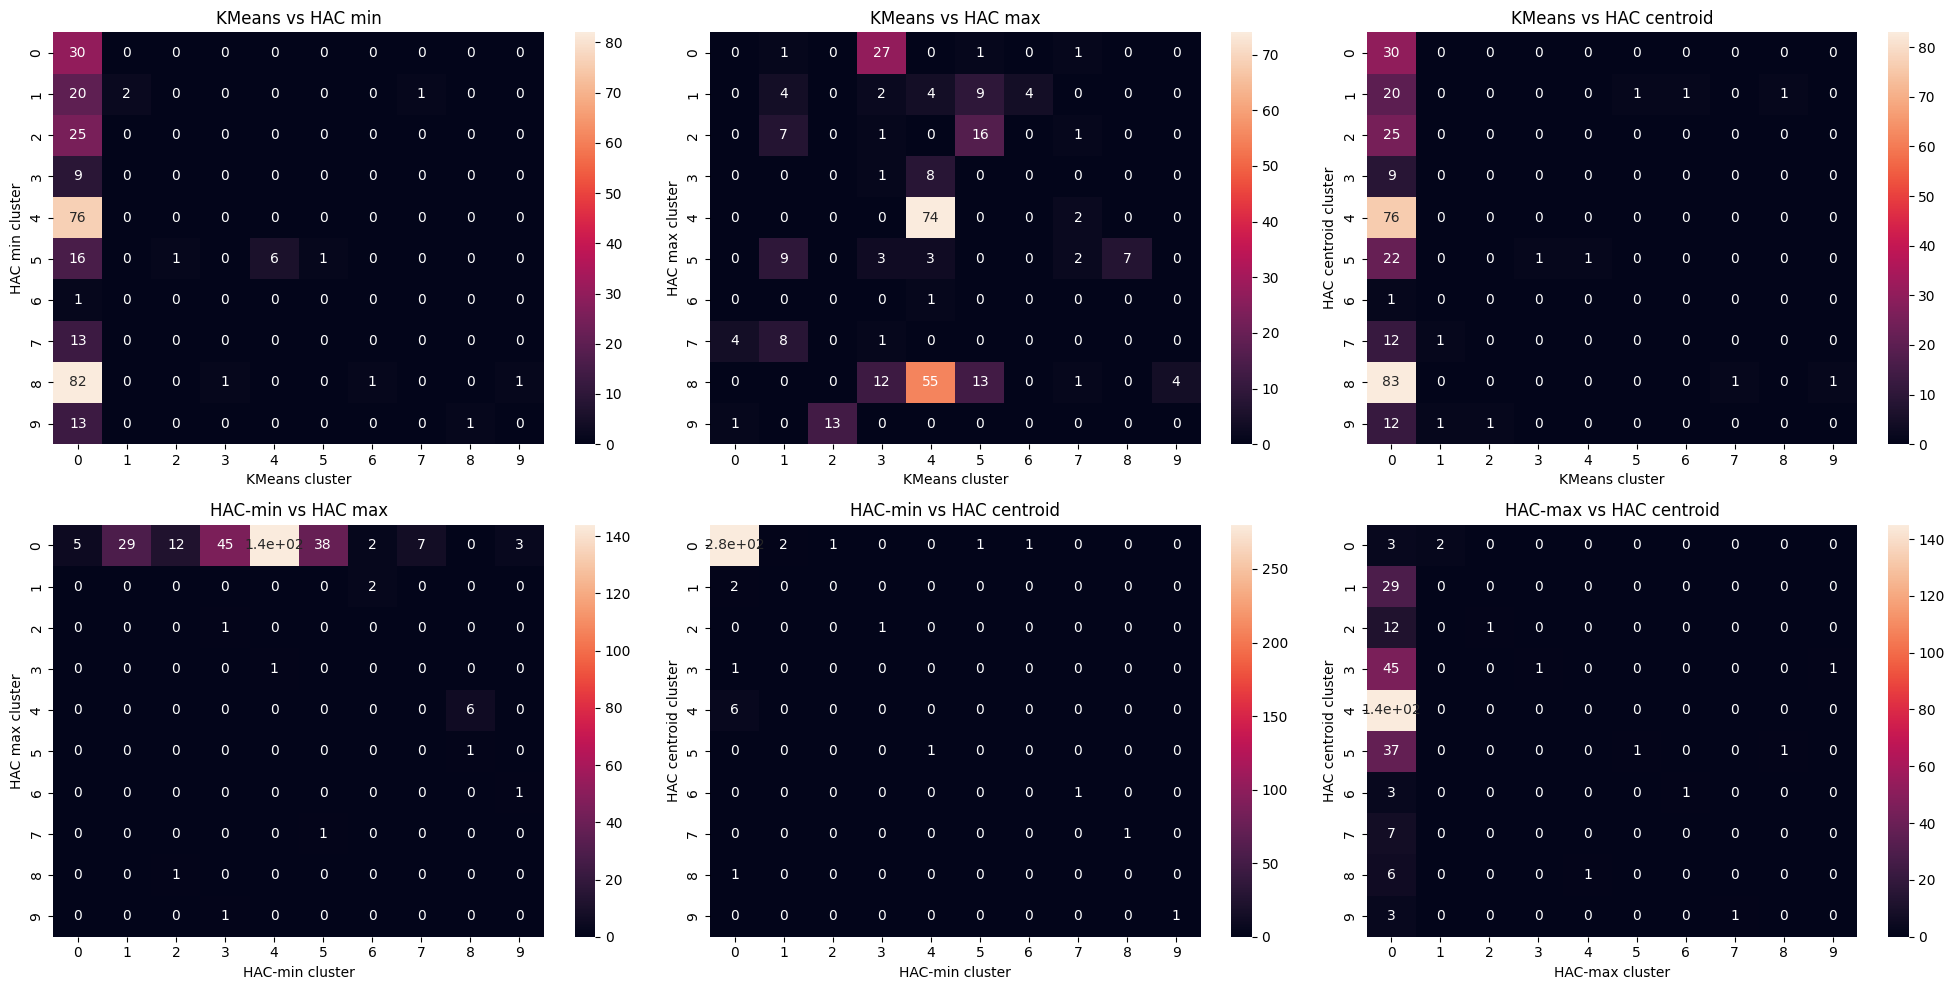
\includegraphics[width=0.9\linewidth]{hw4/img_output/2.6.png}
    \end{figure}
    \textbf{7.} While clustering is useful for exploring data, I do not think it is a good approach for identifying digits. 
    \\
    \\
    (a) Since clustering is unsupervised, it groups images based on overall pixel similarity rather than true digit identity. As a result, I do not expect the clusters to match the actual digit labels. A single digit might be split across several clusters if there is variation in handwriting style, or different digits might end up in the same cluster if they share similar visual features. Thus, using clusters to evaluate or classify digits is inherently limited because the algorithm has no notion of the semantic labels we care about.
    \\
    \\
    (b) Clustering algorithms like K-Means and HAC are sensitive to bad data. If the dataset contains noisy or outlier images -- such as misaligned, heavily smudged, or otherwise unusual examples -- these points can disproportionately influence the formation of clusters. Outliers may either form their own clusters or pull centroids away from the bulk of the data, leading to blurred or unrepresentative mean images. This sensitivity to noisy data further reduces the reliability of clustering for tasks like digit recognition, since it would be very possible for an adversarial attack to insert bad examples and heavily bias the resulting centroids.
\end{solution}


\newpage
%%%%%%%%%%%%%%%%%%%%%%%%%%%%%%%%%%%%%%%%%%%%%
% Problem 3
%%%%%%%%%%%%%%%%%%%%%%%%%%%%%%%%%%%%%%%%%%%%%

\begin{problem}[Ethics Assignment, 5pts]

In the previous problem, you applied K-means and HAC to the MNIST dataset of hand-written digits. In this case, choosing $K=10$ made intuitive sense because we know there are exactly ten digits, and the effectiveness of the clustering algorithm could be easily evaluated. However, clustering is widely used in more complex domains where choosing $K$ is not as straightforward.
\begin{enumerate}
  \item Consider a genetic researcher using clustering algorithms to analyze human genetic sequences. Compare this scenario to the MNIST case. Identify key differences that make selecting the hyperparameter $K$ and evaluating the performance of the algorithms more challenging in genetic research.
  \footnote{This is not a purely fictional case! In 2002, Rosenberg et al. used $K = 6$ in their study of genotypes and human population structure.}
  
  \item Some have argued that because clustering algorithms can group human genetic data into population clusters that roughly align with geographic regions, this supports the idea that racial classifications have a biological basis. Why might this conclusion be premature? Explain why the presence of genetic population clusters alone is not sufficient to establish that humans are divided into distinct biologically significant subgroups (subspecies). You should consider how selection of the hyperparameter $K$ and other model architecture decisions can bias the interpretation of genetic clustering.
  
  \item Finally, discuss one potential harm that could result from drawing such a conclusion too hastily.
\end{enumerate}
\end{problem}

\begin{solution}
    \\
    \textbf{1.} Unlike the MNIST dataset, where the true number of clusters ($K=10$) is known and visually distinguishable, clustering in genetic research lacks a similar kind of clear ground truth. Genetic data is high dimensional, complex, and doesn't have obvious labels like digits. This makes choosing a value of $K$ much more ambiguous -- theres no inherent number of human populations, and the result can change significantly based on the value of $K$. Evaluating performance is also harder, since in MNIST, we can compare clusters to true digit labels for accuracy, but in genetics, there’s no definitive correct way to partition the human genome. This makes validation subjective and dependent on the researchers goals or assumptions.
    \\
    \\
    \textbf{2.} Concluding that racial categories have a biological basis just because genetic clusters align somewhat with geographic regions is premature for several reasons. First, the clustering results are highly sensitive to the chosen $K$. Researchers may select a $K$ that fits their expectations or simplifies interpretation, but this doesn’t mean the resulting clusters are biologically meaningful. Second, clustering algorithms will always produce groupings, even when no real structure exists. This can be problematic as researchers could claim to have found a way to classify all humans into $K$ different types of people. However, in reality, their findings would be because the algorithm was instructed to partition the data into $K$ clusters no matter what, not because of the existence of objectively distinct human subgroups. Finally, most human genetic variation exists within populations, not between them. The appearance of discrete groups could be a result of the method or data sampling, not evidence of biologically distinct subspecies. Race is a social construct with a complex history, and clustering results shouldn’t be used to reinforce outdated or overly simplistic biological narratives.
    \\
    \\
    \textbf{3.} One potential harm of jumping to the conclusion that racial categories are rooted in biology is the misuse of scientific results to justify discrimination and inequality. If people believe that genetics proves the existence of clearly separable groups of humans, then extremists could use this to support a misguided notion of biologically superior or inferior groups. In turn, this can fuel racism, eugenics, and other forms of scientific discrimination. This is not only a perversion of science but also risks serious social and ethical consequences, especially for historically marginalized communities.
\end{solution}

\newpage
%%%%%%%%%%%%%%%%%%%%%%%%%%%%%%%%%%%%%%%%%%%%%
% Name and Calibration
%%%%%%%%%%%%%%%%%%%%%%%%%%%%%%%%%%%%%%%%%%%%%

\textbf{Name}: Jaray Liu

\textbf{Collaborators and Resources}: 

\end{document}
